\documentclass[conference]{ieeetran}
\IEEEoverridecommandlockouts
% The preceding line is only needed to identify funding in the first footnote. If that is unneeded, please comment it out.
%\usepackage{cite}
\usepackage{verbatim}
\usepackage{amsmath,amssymb,amsfonts}
\usepackage{algorithmic}
\usepackage{textcomp}
\usepackage{xcolor}
\def\BibTeX{{\rm B\kern-.05em{\sc i\kern-.025em b}\kern-.08em
    T\kern-.1667em\lower.7ex\hbox{E}\kern-.125emX}}

\usepackage{graphicx}
\graphicspath{ {./res/} }

\usepackage{hyperref}
\usepackage{minted}
\usepackage{flushend}

\newcommand{\norm}[1]{\left\lVert#1\right\rVert}

\begin{document}

\title{Semantic-based Anomaly Detection for \\ Source Code}

\author{\IEEEauthorblockN{
Akimova E.N.\IEEEauthorrefmark{1}\IEEEauthorrefmark{2},
Bersenev A.Yu.\IEEEauthorrefmark{1}\IEEEauthorrefmark{2},
Deikov A.A.\IEEEauthorrefmark{1}\IEEEauthorrefmark{2},
Kobylkin K.S.\IEEEauthorrefmark{1}\IEEEauthorrefmark{2},\\
Konygin A.V.\IEEEauthorrefmark{1},
Mezentsev I.P. \IEEEauthorrefmark{1}\IEEEauthorrefmark{2} and
Misilov V.E.\IEEEauthorrefmark{1}\IEEEauthorrefmark{2}}
\IEEEauthorblockA{
\IEEEauthorrefmark{1}N.N. Krasovskii Institute of Mathematics and Mechanics\\
\IEEEauthorrefmark{2}Ural Federal University\\
Ekaterinburg, Russia \\
Email:
aen15@yandex.ru,
Alexander.Bersenev@urfu.ru,
hx0day@hackerdom.ru,
kobylkinks@gmail.com,\\
konygin@imm.uran.ru,
ilyamezentcev@gmail.com,
v.e.misilov@urfu.ru
}}
\maketitle

\begin{abstract}
In this work, we present a new unsupervised approach to the cross-project code defect prediction.
The code defect prediction problem is formulated as an anomaly detection one.
As a rule, source code anomaly detection problem is treated in the traditional software metrics representation (lines of code, etc.)
 using classical machine learning algorithms (isolation forest, $k$-nearest neighbors algorithm, etc.).
This leads to the fact that the effectiveness of the model depends significantly on the choice of these metrics.
Besides, the total pipeline turns out to be non-differentiable, which makes it difficult to train the pipeline in end-to-end mode.

In our approach, we use the implicit semantic representation of a source code
 and the variational autoencoder for anomaly detection.
Both components are differentiable and can potentially be trained or fine-tuned in end-to-end mode.
The chosen representation of the source code allows one to find atypical, smell, or (potentially) defective code in the semantic space.
In our work, we use a multilingual representation of the source code to detect anomalies in Python programs.
Despite the popularity of this programming language,
 all the works on anomaly detection known to us are devoted to other popular programming languages.
To test the proposed approach, the implemented model was trained and evaluated on the Py150 dataset.
\end{abstract}

\begin{IEEEkeywords}
defect prediction, smell code, anomaly detection, code understanding, variational autoencoder
\end{IEEEkeywords}


\section{Introduction}\label{intro}

Let's say that {\it abnormal} behavior of a program is it state that is {\it not} derived
 from a task this program was originally {\it intended for}.
In other words, a state of a program is not a consequence of an objective, for which the program is developed.
This could have happened for different reasons
\begin{itemize}
\item the program code does not match with the objective;
\item the execution environment does not match with the objective;
\item the input does not match with the objective, and so on.
\end{itemize}
In this work, we will be interested in the program code:
 we split the source code into fragments (code blocks), and find atypical ones among them.
Such atypical fragments are calles  {\it anomalous}, or simply, {\it anomalies}.
Another reason in favor of this terminology is the fact,
 that defects in the code occur as a result of violation of the programming process (see \cite{AfricEtAl2020}).
Also, a strong imbalance of classes (defective and nondefective code) implies that with a suitable representation,
 the potentially defective code may be found as anomalous one (implausible in terms of distribution of the normal code).

In this article, we present a new approach to the cross-project prediction of the source code defects.
The problem of predicting the code defect is posed as a problem of detecting anomalies
 in the semantic multilingual representation of the source code.
Training takes place in an unsupervised mode using the code from different repositories.
The proposed approach is evaluated on the test part of the Py150 dataset.

The rest of the article is organized as follows.
In Section \ref{related}, we discuss existing methods for the source code anomaly detection.
Section \ref{approach} presents our proposed approach to this problem.
Section \ref{results} presents the obtained results.
Section \ref{conclusion} concludes the article by summarizing our results and providing possible directions for the future work.


\section{Background and related work}\label{related}


One of the peculiarities of the defect prediction problem is the imbalance of the classes.
Moreover, creating a big labelled dataset is time consuming and labor intensive.
Together with the progress in machine learning,
 this leads to the fact that the problem of defect code prediction can be posed as a problem of the anomaly detection.
In this case, a way of code representation plays a decisive role.
A code representation is a mapping of code block into a feature vector.
Basically, there are two kinds of features: {\it explicit} and {\it implicit} ones.
Explicit (or {\it traditional}) features are of mostly software metrics.
A more detailed description of these features is given in \cite[Appendix]{AfricEtAl2020}.
The implicit features are generated automatically. 
We will return to the discussion of the code representation in Section \ref{representation}. 

At the moment, the defect code prediction using anomaly detection is becoming more and more popular.
In our opinion, this is due to the progress in deep learning.
In \cite{NeelaEtAl2017}, the authors use explicit features and the Gaussian distribution to model nondefective code.
The defective code is then predicted using the deviation from the model estimation.
The possibility to use explicit features and the $k$-nearest neighbors algorithm
  for the anomaly detection in the source code is demonstrated in \cite{MoshtariEtAl2020}.
In \cite{TongEtAl2018}, the stacked denoising autoencoders are used to extract deep representations from the traditional software metrics.
The similar idea is being implemented in \cite{SakuradaYairi2014} and  \cite{AfricEtAl2020}
 where the autoencoder on the explicit features is used for a within-project source code anomaly detection.
In \cite{BryksinEtAl2020}, two approaches to the code vector representation were implemented:
 a feature vector consisting of $51$ explicit code metrics and an implicit $N$-gram approach.
Several anomaly detection techniques were tested:
 local outlier factor, isolation forest, and autoencoder neural network.
In the study, the authors focus on two types of anomalies: syntax tree anomalies and compiler-induced anomalies in the Kotlin code.

In this work, we use the semantic multilingual embeddings together with a variational autoencoder to detect anomalies in the Python code.
To the best of our knowledge, we are the first to propose such model.

\section{The proposed approach}\label{approach}

We use the unlabelled dataset of source code, which leads us to unsupervised anomaly detection methods.
The proposed approach is as follows.
First, we calculate the semantic contextual multilingual embeddings to represent the code blocks.
Secondly, we use the variational autoencoder as an anomaly detector.
A variational autoencoder allows us to obtain not only an estimate for the code anomality, but, also, a probabilistic model.
Also, the variational autoencoder can be combined with the neural network that is used for the code representation.
It gives a possibility to fine-tune the model in end-to-end mode.

The reconstruction error of an unseen samples of the code blocks will have a certain probability of belonging to the negative reconstruction error distribution,
 and a certain probability of belonging to the positive reconstruction error distribution.
Based on those probabilities, we classify the samples as nondefective or defective.

The proposed approach for the code anomaly detection at a scale consists of the following steps:
\begin{enumerate}
\item retrieve a large representative corpora of source code;
\item extract features (calculate embeddings);
\item run anomaly detection;
\item process the output of the anomaly detection algorithm. 
\end{enumerate}


\subsection{Dataset}

In the present work, the dataset Py150 (see \cite{RaychevEtAl2016}) is used.
The dataset consists of the Python programs that were collected from the GitHub\footnote{https://github.com/} repositories
 by removing duplicate files, removing project forks (copy of another existing repository),
 keeping only programs that parse and have at most 30'000 nodes in the AST (abstract syntax tree).
Furthermore, only repositories with the permissive and non-viral licenses such as MIT, BSD, and Apache were used.
The dataset is split into two parts -- 100'000 files used for training and 50'000 files used for evaluation. 

For our purposes, we need to extract code blocks from the Py150.
The code blocks, in our case, are the functions that we found with \texttt{ast}\footnote{https://docs.python.org/3/library/ast.html} package.
Every such code block correspods to a node in AST and has type \texttt{ast.FunctionDef} or \texttt{ast.AsyncFunctionDef}.
As a result, we got about one million code blocks --- inputs for the proposed model.

We use the train/test split for the code blocks induced by the original train/test split for the Python programs in Py150.


\subsection{Code representation}\label{representation}

The next step in our approach is to calculate the vector representations (embeddings) for the code blocks.
There are many different ways to get a vector representation of a code block,
 e.g.  code2vec, code2seq, PathPair2Vec, CuBERT, CodeBERT
 (see \cite{AlonEtAl2019vec}, \cite{AlonEtAl2019seq},  \cite{ShiEtAl2020}, \cite{KanadeEtAl2020}, \cite{FengEtAl2020}), and so on.
The proposed approach uses the CodeBERT model.
It is a bimodal pre-trained model for a  natural language and the following programming languages:
  Python, Java, JavaScript, PHP, Ruby, Go.
The model follows BERT (see \cite{DevlinEtAl2019}) and RoBERTa (see \cite{LiuEtAl2019}),
 and uses the multi-layer bidirectorial Transformer (see \cite{VaswaniEtAl2017}) as the model architecture
 (see Fig. \ref{bert_arch}\footnote{The source of the image is the article \texttt{http://jalammar.github.io/illustrated-bert/}}).
\begin{figure}[htbp]
\caption{BERT architecture.
Just like the encoder of the Transformer,
 BERT takes a sequence of words as input which keep flowing up the stack.
 Each layer applies self-attention, and passes its results through a feed-forward network, and then hands it off to the next encoder.}
\centering
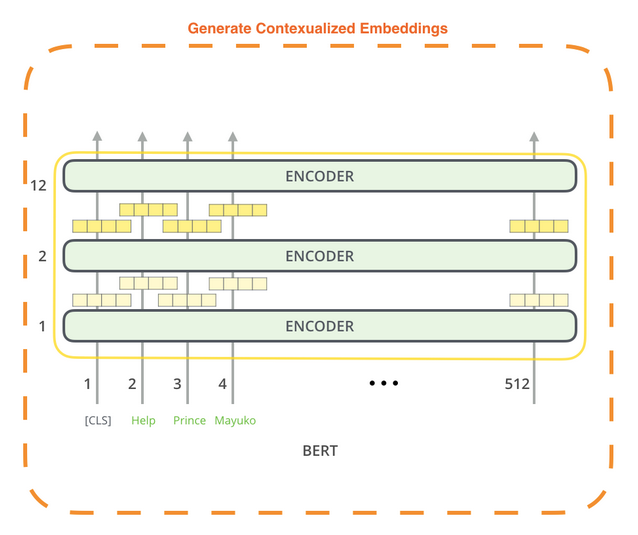
\includegraphics[width=0.5\textwidth]{bert_arch}
\label{bert_arch}
\end{figure}
CodeBERT captures the semantic connection between the natural language and programming language
 and produces the general-purpose representations that can broadly support NL-PL understanding tasks
 (e.g. natural language code search) and generation tasks (e.g. code documentation generation).
CodeBERT is trained on two objectives: Masked Language Modeling and Replaced Token Detection.
Due to the architecture and learning method, CodeBERT allows one to get the contextual semantic embeddings.
As a result, the representation of a fragment depends more on the semantics and less on syntax.
In this work, we used a pre-trained model from the \texttt{Huggingface}\footnote{https://huggingface.co/microsoft/codebert-base}.
It is based on \texttt{RobertaModel}\footnote{https://huggingface.co/transformers/model\_doc/roberta.html} --- a model proposed in \cite{LiuEtAl2019}.
The resulting embedding is the $768$-dimensional outputs from the penultimate layer of the Transformer.
We experimented with other layers, but the penultimate layer turned out to be the most suitable:
 on the one hand, it contains the high-level information,
 on the other hand, it is not as well trained for the pre-training tasks as the last layer). 


\subsection{Anomaly detection}

For the anomaly detection the model uses variational autoenconder (see \cite{KingmaWelling2014, RezendeEtAl2014}).
In the variational autoencoder, the loss function is composed of two parts:
 the $L_2$-loss (generative loss) and Kullback --- Leibler divergence (latent loss, see \cite[Appendix B]{KingmaWelling2014}):
$$\norm{X - f(z)} + \mathcal{KL}[\mathcal{N}(\mu(X), \Sigma(X) ) || \mathcal{N}(0, I)].$$
Unlike a simple autoencoder, a variational autoencoder can approximate by virtue of the Bayesian inference.
This leads to the fact, that a variational autoencoder is more appropriate for the extrapolation tasks than a simple autoencoder.
A diagram of the variational autoencoder is given
 in Fig. \ref{vae_gaussian_arch}\footnote{The source of the image is the preprint by C. Doersch ``Tutorial on variational autoencoders'', 2016.}.

\begin{figure}[htbp]
\caption{Variational autoencoder. Left is without the ``reparameterization trick'', and right is with it.
Red shows sampling operations that are non-differentiable.
Blue shows loss layers.
The feedforward behavior of these networks is identical, but backpropagation can be applied only to the right network.
}
\centering
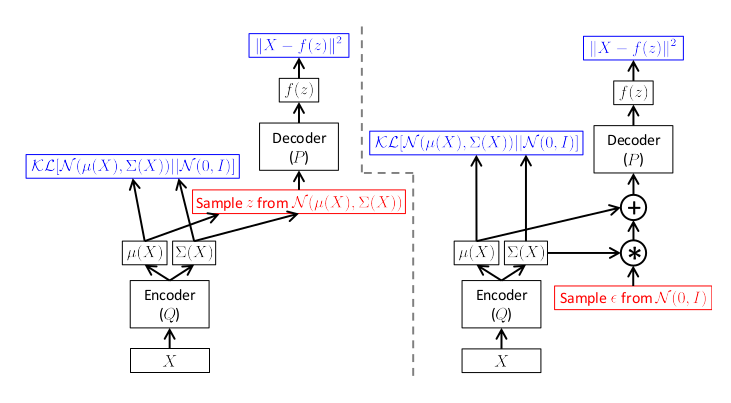
\includegraphics[width=0.5\textwidth]{vae_gaussian_arch}
\label{vae_gaussian_arch}
\end{figure}

The variational autoencoder describes the latent space in terms of probability distribution.
The encoding that has been learned by autoencoder so far describes a sample draw from some latent space
 determined by the encoder.
The variational autoencoder learns to represent the encoding as latent distributions
 instead of each value of the encoding being represented by a single value as the other autoencoders have done so far,

The parameters of our variational autoencoder were learned with respect to the Gaussian distribution.
The hidden state size is equal to $20$.

\section{Results}\label{results}

The Py150 train/test split gives us about $641$ thousands datapoints in train and about $314$ thousands datapoints in test.
Every datapoint is represented by $768$-dimensional embedding.
Obtaining such a representation does not require training, since we are using a model with pre-trained weights. 
However the proposed approach leaves a possibility to fine-tune the code representation model for downstream tasks.

In the next step, we trained the variational autoencoder.
Training took place over $200$ epochs, as an optimization algorithm were used Adam (see \cite{KingmaBa2015}) with learning rate $0.001$ 
and batch size $128$.

The resulting model allows to predict the anomalousness of a code block.
The reconstruction loss of the variational autoencoder provides such prediction:
the larger the reconstruction loss, the less likely the code block  is ``typical'',
 therefore, the more likely the code block is abnormal.

To the best of our knowledge, there are no public datasets in which abnormal code block would be labelled. 
To evaluate the model we use the unlabelled test part of Py150 dataset.
Test code has been removed.
The distribution of reconstruction losses is given in Fig. \ref{reconstruction_loss}. 

\begin{figure}[htbp]
\caption{Reconstruction loss.
The picture shows the distribution of reconstruction losses on test part from the Py150 dataset.
The horizontal axis corresponds to the loss value.
The vertical axis is the number of code blocks.}
\centering
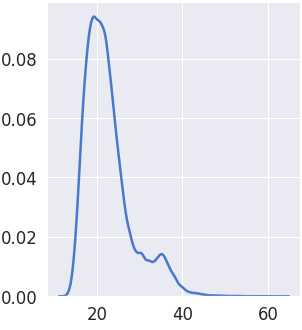
\includegraphics[width=0.3\textwidth]{reconstruction_loss}
\label{reconstruction_loss}
\end{figure}

Thus, the model outputs corresponding to a large reconstruction error (right-hand side) are anomalies,
 i.e., code blocks that implement rare (but correct) logic
 or (potentially) defective code blocks.
Full list of code blocks from the test part of the Py150 dataset with a reconstruction loss of more than $35.0$
 is given in \url{https://github.com/konygin/code_anomaly_detection}.
The samples are supplied with the path in the corresponding repository and line numbers.

For convenience, we provide a few examples below.
We have tried to select compact anomalous code blocks that implement different logic.


\begin{minted}[fontsize=\footnotesize,
               frame=lines,
               mathescape,
               framesep=5mm]{python}
def __SOCKADDR_COMMON(sa_prefix): return \
\end{minted}

\begin{minted}[fontsize=\footnotesize,
               mathescape,
               framesep=5mm]{python}
def Pop(): pass
\end{minted}

\begin{minted}[fontsize=\footnotesize,
               mathescape,
               frame=lines,
               framesep=5mm]{python}
def read( targetfile):
  code =  r"\x31\xc0\x50\x50\xb0\x17\xcd\x80\xeb\x1f"
  code += r"\x5e\x50\x68\x2f\x63\x61\x74\x68\x2f\x62"
  code += r"\x69\x6e\x89\xe3\x50\x56\x53\x89\xe2\x50"
  code += r"\x52\x53\xb0\x3b\x50\xcd\x80\x50\x50\xcd"
  code += r"\x80\xe8\xdc\xff\xff\xff"
  code += targetfile
  return code
\end{minted}

\begin{minted}[fontsize=\footnotesize,
               mathescape,
               framesep=5mm]{python}
def L_(s):
  return s
\end{minted}

\begin{minted}[fontsize=\footnotesize,
               mathescape,
               frame=lines,
               framesep=5mm]{python}
def __init__(self):
  self.data_link = 'aHR0cHM6Ly9vZmZzaG9yZWdpdC5jb20\
  vbGFtYmRhODEvZGF0YWJhc2VzL21vdmllZmFyc2kuemlw'
\end{minted}

\begin{minted}[fontsize=\footnotesize,
               mathescape,
               framesep=5mm]{python}
def create_ruby_dpowerline():
  vim.command((
    '''
    ruby
    if $powerline == nil
      class Powerline
      end
      $powerline = Powerline.new
    end
    '''
  ))
\end{minted}

\begin{minted}[fontsize=\footnotesize,
               mathescape,
               frame=lines,
               framesep=5mm]{python}
def HRESULT_SEVERITY(hr):
  return (((hr) >> 31) & 1)
\end{minted}

\begin{minted}[fontsize=\footnotesize,
               mathescape,
               framesep=5mm]{python}
def stream():
  yield ''
\end{minted}

\begin{minted}[fontsize=\footnotesize,
               mathescape,
               frame=lines,
               framesep=5mm]{python}
def IN_CLASSA(a):
  return ((((in_addr_t)(a)) & (-2147483648)) == 0)
\end{minted}

\begin{minted}[fontsize=\footnotesize,
               mathescape,
               framesep=5mm]{python}
def __init__(self, root):
  self._root = root
  self._invalids = set(['hamshahri.dtd',  \
    'HAM2-960622.xml', 'HAM2-960630.xml', \
    'HAM2-960701.xml', 'HAM2-960709.xml', \
    'HAM2-960710.xml', 'HAM2-960711.xml', \
    'HAM2-960817.xml', 'HAM2-960818.xml', \
    'HAM2-960819.xml', 'HAM2-960820.xml', \
    ... # code omitted for brevity
    'HAM2-050407.xml', 'HAM2-050416.xml'])
  self._paragraph_pattern = \
    re.compile(r'(\n.{0,50})(?=\n)')
\end{minted}

\begin{minted}[fontsize=\footnotesize,
               mathescape,
               frame=lines,
               framesep=5mm]{python}
def isspace(c):
  return _ctoi(c) in (9, 10, 11, 12, 13, 32)
\end{minted}

\begin{minted}[fontsize=\footnotesize,
               mathescape,
               framesep=5mm]{python}
def setKr(a):
  global m_Kr, m_Kr4PI, fKrESun
  m_Kr = a
  m_Kr4PI = m_Kr*4.0*math.pi
  fKrESun = m_Kr * m_ESun
\end{minted}

\begin{minted}[fontsize=\footnotesize,
               mathescape,
               frame=lines,
               framesep=5mm]{python}
def ali_decode(letter):
  t=maketrans("qwertyuiopasdfghjklzxcvbnm",\
    "abcdefghijklmnopqrstuvwxyz")
  return letter.translate(t)
\end{minted}

\begin{minted}[fontsize=\footnotesize,
               mathescape,
               framesep=5mm]{python}
def escape(value):
  return str(value).replace('\\', '\\\\').\
    replace(':', '\\:').replace(' ', '-')
\end{minted}

\begin{minted}[fontsize=\footnotesize,
               mathescape,
               frame=lines,
               framesep=5mm]{python}
def p_term(p):
        '''term : age_term
                | recentlyseen_term
                | change_term
                | owner_term
                | reviewer_term
                | commit_term
                | project_term
                | project_key_term
                | branch_term
                | topic_term
                | ref_term
                | label_term
                | message_term
                | comment_term
                | has_term
                | is_term
                | status_term
                | file_term
                | limit_term
                | op_term'''
        p[0] = p[1]
\end{minted}


\section{Conclusion}\label{conclusion}

We present a new approach to the cross-project prediction of the source code defects.
The problem of predicting a code defect is posed as a problem of detecting anomalies using a variational
 autoencoder for the semantic multilingual representation of the source code.
Training takes place in an unsupervised mode and uses the code from different projects.
The variational autoencoder can be combined with the neural network that is used for code representation.
It gives a possibility to fine-tune the model in the end-to-end mode.

In our future work, we will aim to train the multilingual variational autoencoder.
It leads to a multilingual anomaly detection model.
Besides, we will aim to use the generative abilities of the  variational autoencoder to interpret the detected anomalies.
We plan to make the model publicly available. 

%This research has been supported by Huawei.
%Special thanks to the System Programming Laboratory (Huawei RRI).
Computations were performed on the Uran supercomputer at the IMM UB RAS.

\begin{thebibliography}{00}
\bibitem{AfricEtAl2020}
 P. Afric, L. Sikic, A. Kurdija, S. Adrian, and M. Silic,
 ``REPD: Source code defect prediction as anomaly detection'',
 J. Syst. Softw., vol. 168, 2020.

\bibitem{AllamanisEtAl2018}
 M. Allamanis, E.T. Barr, P. Devanbu, Ch. Sutton,
 ``A Survey of Machine Learning for Big Code and Naturalness'',
 ACM Comput. Surv., vol. 51, no. 4, 2018.

\bibitem{AlonEtAl2019vec}
 U. Alon, M. Zilberstein, O. Levy, and E. Yahav,
 ``Code2vec: Learning distributed representations of code'',
 Proc. ACM Program. Lang., vol. 3, 2019.

\bibitem{AlonEtAl2019seq}
 U. Alon, Sh. Brody, O. Levy, and E. Yahav,
 ``code2seq: Generating sequences from structured representations of code'',
 ICLR'19, 2019.

\bibitem{BryksinEtAl2020}
 T. Bryksin, V. Petukhov, I. Alexin, S. Prikhodko, A. Shpilman, V. Kovalenko, and  N. Povarov,
 ``Using large-scale anomaly detection on code to improve Kotlin compiler'',
 Proc. MSR, pp. 455--465, 2020.

\bibitem{DevlinEtAl2019}
 J. Devlin, M.-W. Chang, K. Lee, and K. Toutanova,
 ``BERT: Pre-training of deep bidirectional transformers for language understanding'',
 Proc. NAACL, pp. 4171--4186, 2019.

\bibitem{FengEtAl2020}
 Zh. Feng, D. Guo, D. Tang, N. Duan, X. Feng, M. Gong, L. Shou, B. Qin, T. Liu, D. Jiang, and M. Zhou,
``CodeBERT: A pre-trained model for programming and natural languages'',
 Findings of the Association for Computational Linguistics: EMNLP 2020, pp. 1536--1547, 2020.

\bibitem{KanadeEtAl2020}
 A. Kanade, P. Maniatis, G. Balakrishnan, and K. Shi,
 ``Learning and evaluating contextual embedding of source code'',
 Proc. MLR, vol. 119, pp. 5110--5121, 2020.

\bibitem{KingmaBa2015}
 D.P. Kingma, J. Ba,
 ``Adam: A method for stochastic optimization'',
 Proc. ICLR, 2015.

\bibitem{KingmaWelling2014}
 D.P. Kingma, M. Welling,
 ``Auto-encoding variational Bayes'',
 Proc. ICLR, 2014.

\bibitem{LiuEtAl2019}
 Y. Liu, M. Ott, N. Goyal, J. Du, M. Joshi, D. Chen, O. Levy, M. Lewis, L. Zettlemoyer, and V. Stoyanov,
 ``RoBERTa: A robustly optimized BERT pretraining approach'',
 arXiv:1907.11692 [cs], Jul. 2016.

\bibitem{MoshtariEtAl2020}
 S. Moshtari, J.C.S. Santos, M. Mirakhorli, and A. Okutan,
 ``Looking for software defects? First find the nonconformists'',
 2020 IEEE 20th International Working Conference on Source Code Analysis and Manipulation (SCAM), Adelaide, SA, Australia, 2020, pp. 75--86, doi: 10.1109/SCAM51674.2020.00014 .

\bibitem{NeelaEtAl2017}
 K.N. Neela, S.A. Ali, A.S. Ami, and A.U. Gias,
 ``Modeling software defects as anomalies: a case study on Promise repository'',
 J. Softw., vol.12, no. 10, pp. 759--772, 2017.

\bibitem{RaychevEtAl2016}
V. Raychev, P. Bielik, and M. Vechev,
 ``Probabilistic model for code with decision trees'',
 SIGPLAN Not. vol. 51, nov. 10, pp. 731--747, 2016, doi: 10.1145/3022671.2984041 .

\bibitem{RezendeEtAl2014}
 D.J. Rezende, Sh. Mohamed, and D. Wierstra,
 ``Stochastic backpropagation and approximate inference in deep generative models'',
  Proceedings of the 31st International Conference on Machine Learning, PMLR vol. 32, no. 2, pp. 1278--1286, 2014. 

\bibitem{SakuradaYairi2014}
 M. Sakurada, T. Yairi,
 ``Anomaly detection using autoencoders with nonlinear dimensionality reduction'',
 In Proceedings of the MLSDA 2014 2nd Workshop on Machine Learning for Sensory Data Analysis (MLSDA'14).
 Association for Computing Machinery, New York, NY, USA, pp. 4--11. doi: 10.1145/2689746.2689747 .

\bibitem{ShiEtAl2020}
 K. Shi, Y. Lu, J. Chang, and Zh. Wei,
 ``PathPair2Vec: An AST path pair-based code representation method for defect prediction'',
 Journal of Computer Languages, vol. 59, 2020. doi: 10.1016/j.cola.2020.100979 .

\bibitem{TongEtAl2018}
 H. Tong, B. Liu, and Sh. Wang,
 ``Software defect prediction using stacked denoising autoencoders and two-stage ensemble learning'',
 Information and Software Technology, vol. 96, pp. 94--111, 2018. doi: 10.1016/j.infsof.2017.11.008 .

\bibitem{VaswaniEtAl2017}
 A. Vaswani, N. Shazeer, N. Parmar, J. Uszkoreit, L. Jones, A.N. Gomez, \L. Kaiser, and I. Polosukhin,
 ``Attention is all you need'',
 Proceedings of the 31st International Conference on Neural Information Processing Systems, pp. 6000--6010, 2017.

\end{thebibliography}

\end{document}
